\documentclass{article}

\usepackage[nottoc]{tocbibind}
\usepackage[a4paper, total={7.7in, 11in}]{geometry}
\usepackage[utf8]{inputenc}
\usepackage{amsmath,amssymb}
\usepackage{chngpage}
\usepackage{graphicx}
\DeclareMathOperator{\E}{\mathbb{E}}
\DeclareMathOperator{\D}{\mathbb{D}}

\begin{document}

\title{Machine Learning Project 2018: With Cherry Flavor}
\maketitle

\small

\section{Introduction}

Indoor  navigation  and  collision  avoidance  is  one  of  the
basic  requirements  for  robotic  systems  that  must  operate  in
unstructured  open-world  environments,  including  quadrotors,
mobile  manipulators,  and  other  mobile  robots.  Many  of  the
most successful approaches to indoor navigation have used
mapping  and  localization  techniques  based  on  3D
perception,  including  SLAM,  depth  sensors,  stereo  cameras,
and  monocular  cameras  using  structure  from  motion.
The use of sophisticated sensors and specially mounting multiple
cameras on the robot imposes additional costs on
a  robotic  platform,  which  is  a  particularly  prominent  issue
for weight and power constrained systems such as lightweight
aerial vehicles. Monocular cameras, on the other hand, require
3D  estimation  from  motion,  which  remains  a  challenging
open  problem  despite  considerable  recent  progress.
In this project we are based on the paper \cite{cad2rl},
and explore a learning-based approach for indoor
navigation,  which  directly  predicts  collision-free
commands from monocular images, without attempting to
explicitly  model  or  represent  the  3D  structure
of  the  environment.

To model the environment, we use Unreal Engine and AirSim.

\subsection{Unreal Engine}

The Unreal Engine is a game engine developed by Epic Games,
first showcased in the 1998 first-person shooter game Unreal.
Although primarily developed for first-person shooters, it has
been successfully used in a variety of other genres, including
stealth, fighting games, MMORPGs, and other RPGs. With its code
written in C++, the Unreal Engine features a high degree of portability
and is a tool used by many game developers today. It has won several
awards, including the Guinness World Records award
for "most successful video game engine."

\subsection{AirSim}

Recently, paradigms such as reinforcement learning, learning-by-demonstration
and transfer learning are proving a natural means to train various robotics
systems. One of the key challenges with these techniques is the high sample
complexity - the amount of training data needed to learn useful behaviors is often
prohibitively high. This issue is further exacerbated by the fact that autonomous
vehicles are often unsafe and expensive to operate during the training phase. In order to
seamlessly operate in the real world, the robot needs to transfer the learning it does
in simulation. Currently, this is a non-trivial task as simulated perception, environments
and actuators are often simplistic and lack the richness or diversity of the
real world. For example, for robots that aim to use computer vision in outdoor
environments, it may be important to model real-world complex objects such as trees,
roads, lakes, electric poles and houses along with rendering that includes finer
details such as soft shadows, specular reflections, diffused inter-reflections and so on.
Similarly, it is important to develop more accurate models of system dynamics so
that simulated behavior closely mimics the real-world.

AirSim  is  an  open-source  platform \cite{airsim2017fsr} by Microsoft,
that  aims  to  narrow  the  gap  between
simulation  and  reality  in  order  to
aid  development  of  autonomous  vehicles.
The platform is based on the Unreal Engine, and seeks to positively
influence development and testing of data-driven
machine intelligence techniques such as reinforcement learning and
deep learning. It is inspired by several previous simulators (see
related work), and proved to be very useful in this project development.

\section{Project description and approach using Reinforcement Learning}

The project is about collision avoidance in AirSim +
UnrealEngine environment, using deep reinforcement learning.

{\bf Reinforcement learning }(RL) is an area of machine learning inspired
by behaviorism, concerned with how agents ought to take actions in an
environment so as to maximize some notion of cumulative reward.
The problem, due to its generality, is studied in many other disciplines,
such as game theory, control theory, operations research, information theory,
simulation-based optimization, multi-agent systems, swarm intelligence,
statistics and genetic algorithms. In the operations research and
control literature, reinforcement learning is called approximate dynamic
programming. The approach has been studied in the optimal control theory,
though most studies are concerned with the existence of optimal
solutions and their characterization, and not with learning or approximation.

{\bf $Q$-learning} is a model-free reinforcement learning technique.
It is able to compare the expected utility of the available actions
(for a given state) without requiring a model of the environment.
Additionally, $Q$-learning can handle problems with stochastic
transitions and rewards, without requiring adaptations.

It has been proven that for any finite Markov decision process (MDP),
$Q$-learning eventually finds an optimal policy, in the sense that the
expected value of the total reward return over all successive steps,
starting from the current state, is the maximum achievable.

Specifically, $Q$-learning can identify an optimal
action-selection policy for any given (finite) MDP.
It works by learning an action-value function $Q(s, a)$, which
ultimately gives the expected utility of a given action $a$
while in a given state $s$ and following an optimal policy thereafter.
A policy $\pi$, is a rule that the agent follows in selecting actions,
given the state it is in. When such an action-value function is learned,
the optimal policy can be constructed by selecting
the action with the highest value in each state.

The problem space consists of an agent, a set of states $S$,
and a set of actions per state $A$. By performing an action $a \in A$,
the agent can move from state to state. Executing an action in a
specific state provides the agent with a reward (a numerical score).
The goal of the agent is to maximize its total (future) reward.
It does this by learning which action is optimal for each state.
The action that is optimal for each state is the action that has
the highest long-term reward. This reward is a weighted sum of
the expected values of the rewards of all future steps starting from
the current state, where the weight for a step from a state $\Delta t$
steps into the future is calculated as $\gamma^{\Delta t}$.
Here, $\gamma$ is a number between 0 and 1 ($0 \le \gamma \le 1$) called
the {\it{discount factor}} and trades off the importance of earlier
versus later rewards. $\gamma$ may also be interpreted as the
probability to succeed (or survive) at every step $\Delta t$.

The algorithm, therefore, has a function that calculates
the quality of a state-action combination:

$$Q: S \times A \to \mathbb{R}$$

Before learning begins, $Q$ is initialized to a possibly arbitrary fixed value.
Then, at each time $t$, the agent selects an action $a_t$, observes a reward $r_t$,
enters a new state $s_{t+1}$ (that may depend on both the previous state $s_t$
and the selected action), and $Q$ is updated.

$$Q(s_{t},a_{t}) \leftarrow (1-\alpha) \cdot
\underbrace{Q(s_{t},a_{t})}_{\rm old~value} +
\underbrace{\alpha}_{\rm learning~rate} \cdot
\overbrace{\bigg( \underbrace{r_{t}}_{\rm reward} +
\underbrace{\gamma}_{\rm discount~factor} \cdot
\underbrace{\max_{a}Q(s_{t+1}, a)}_{\rm
estimate~of~optimal~future~value} \bigg) }^{\rm learned~value} $$

where $r_{t}$ is the reward observed for the current state
$s_t$, and $\alpha$ is the learning rate.


\section{Description of the framework architecture}

Architecture consists of the following classes. The main character is
Agent, which can act, observe and train.
To make agent more readable, we separated History and
ExperienceReplayMemory into separated classes.
With the goal of making substitutable actions and rewards,
we introduced classes ActionSpace and Reward.
To control exploration-exploatation dilemma, we created module to
handle exploration (with Explorer classes).

Our implementation uses deep learning libraries CNTK
and TensorFlow (with Tensorboard).

\section{Considered Environments}

The following environments were considered under Linux:
\begin{enumerate}
    \item Blocks.
    \item Cave.
    \item Landscape Mountains.
    \item Corridor.
\end{enumerate}

 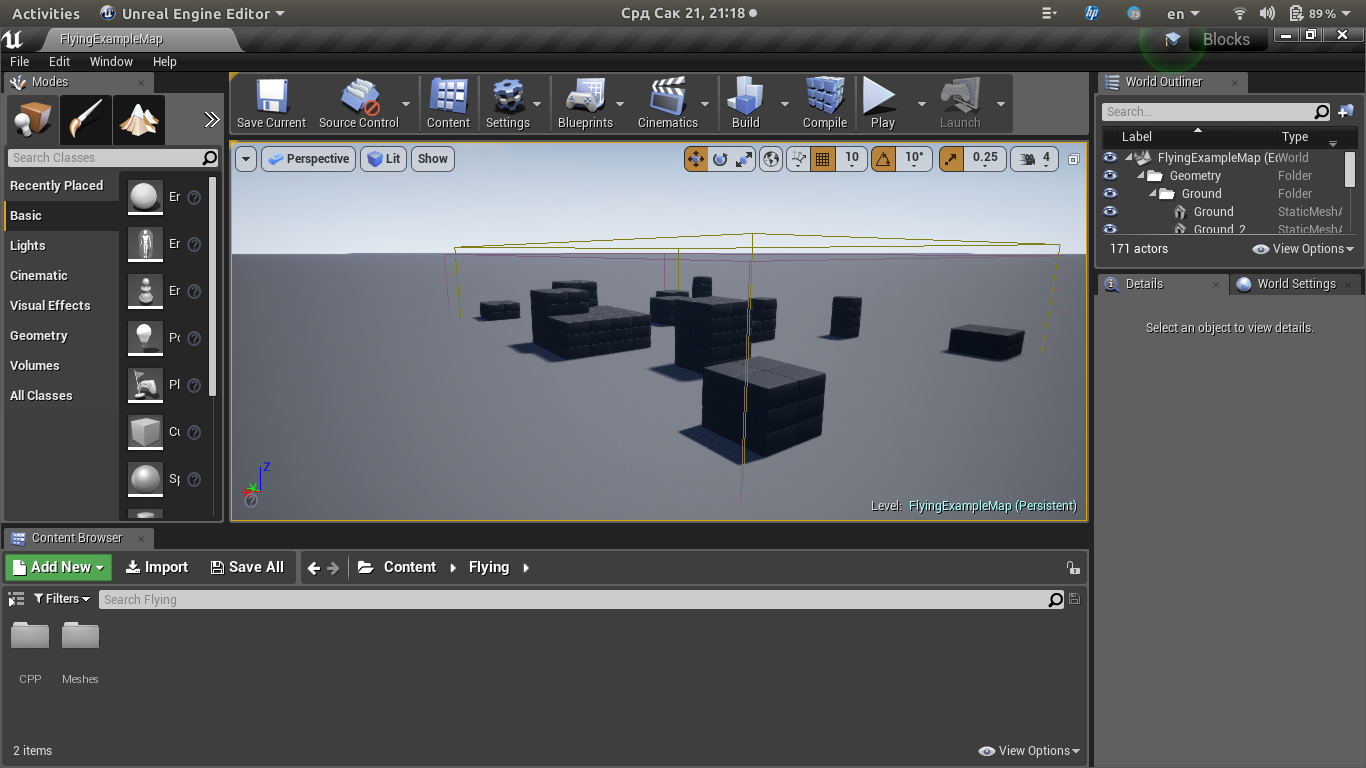
\includegraphics[scale=0.1]{environments/blocks.png}
 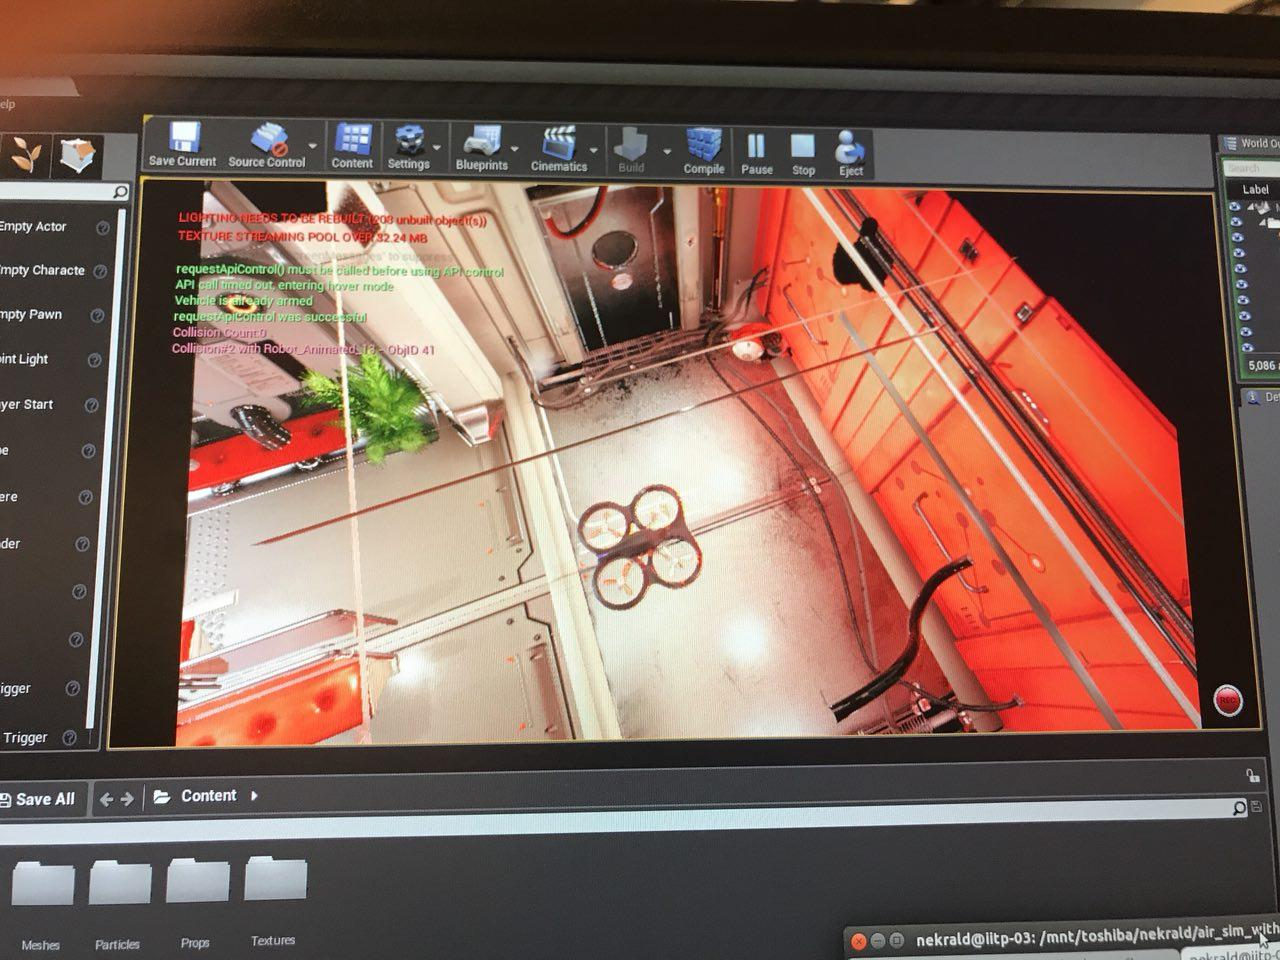
\includegraphics[scale=0.1]{environments/corridor.jpg}
 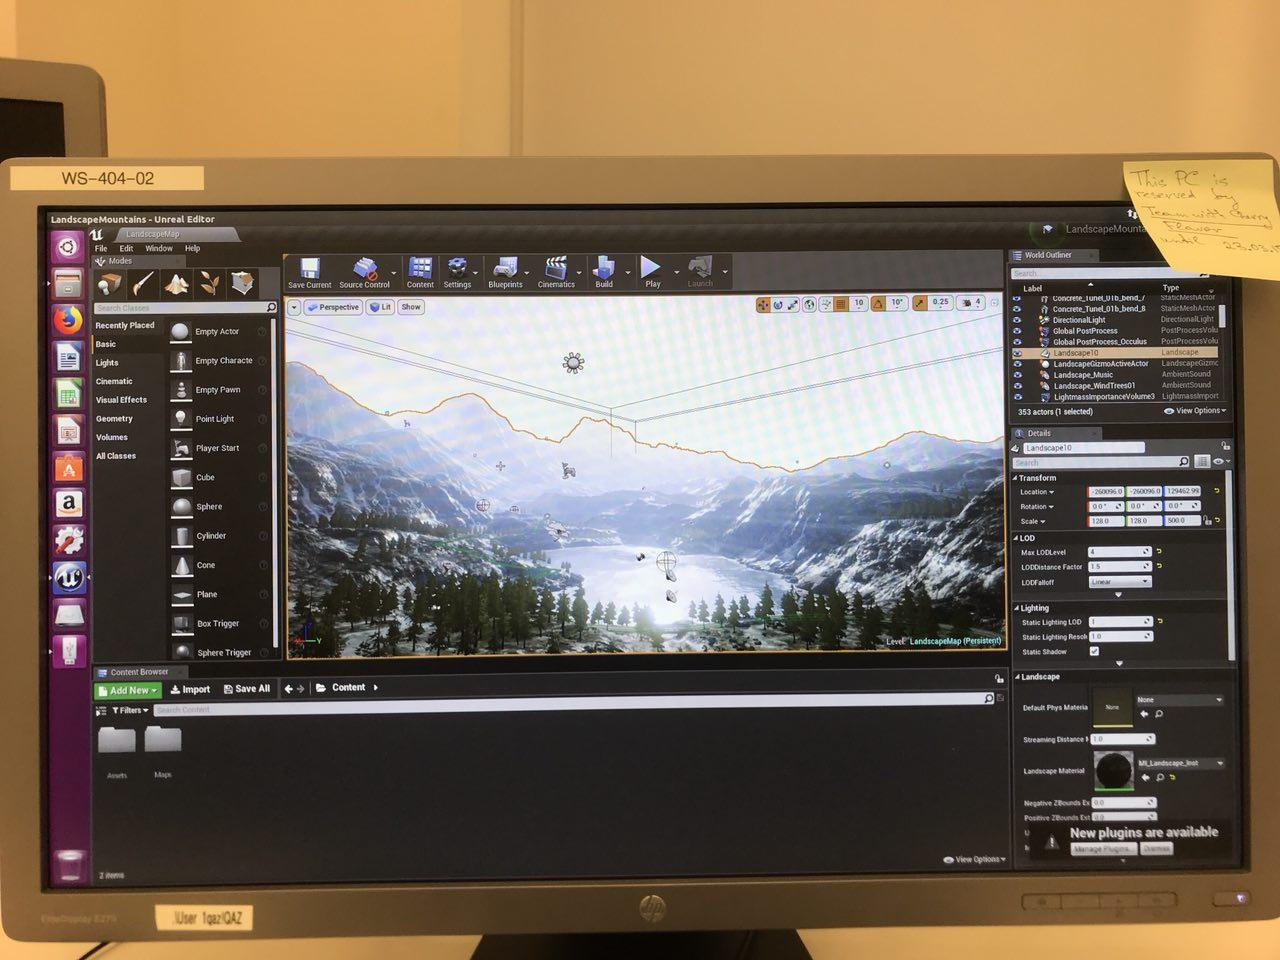
\includegraphics[scale=0.1]{environments/landscape.jpg}
 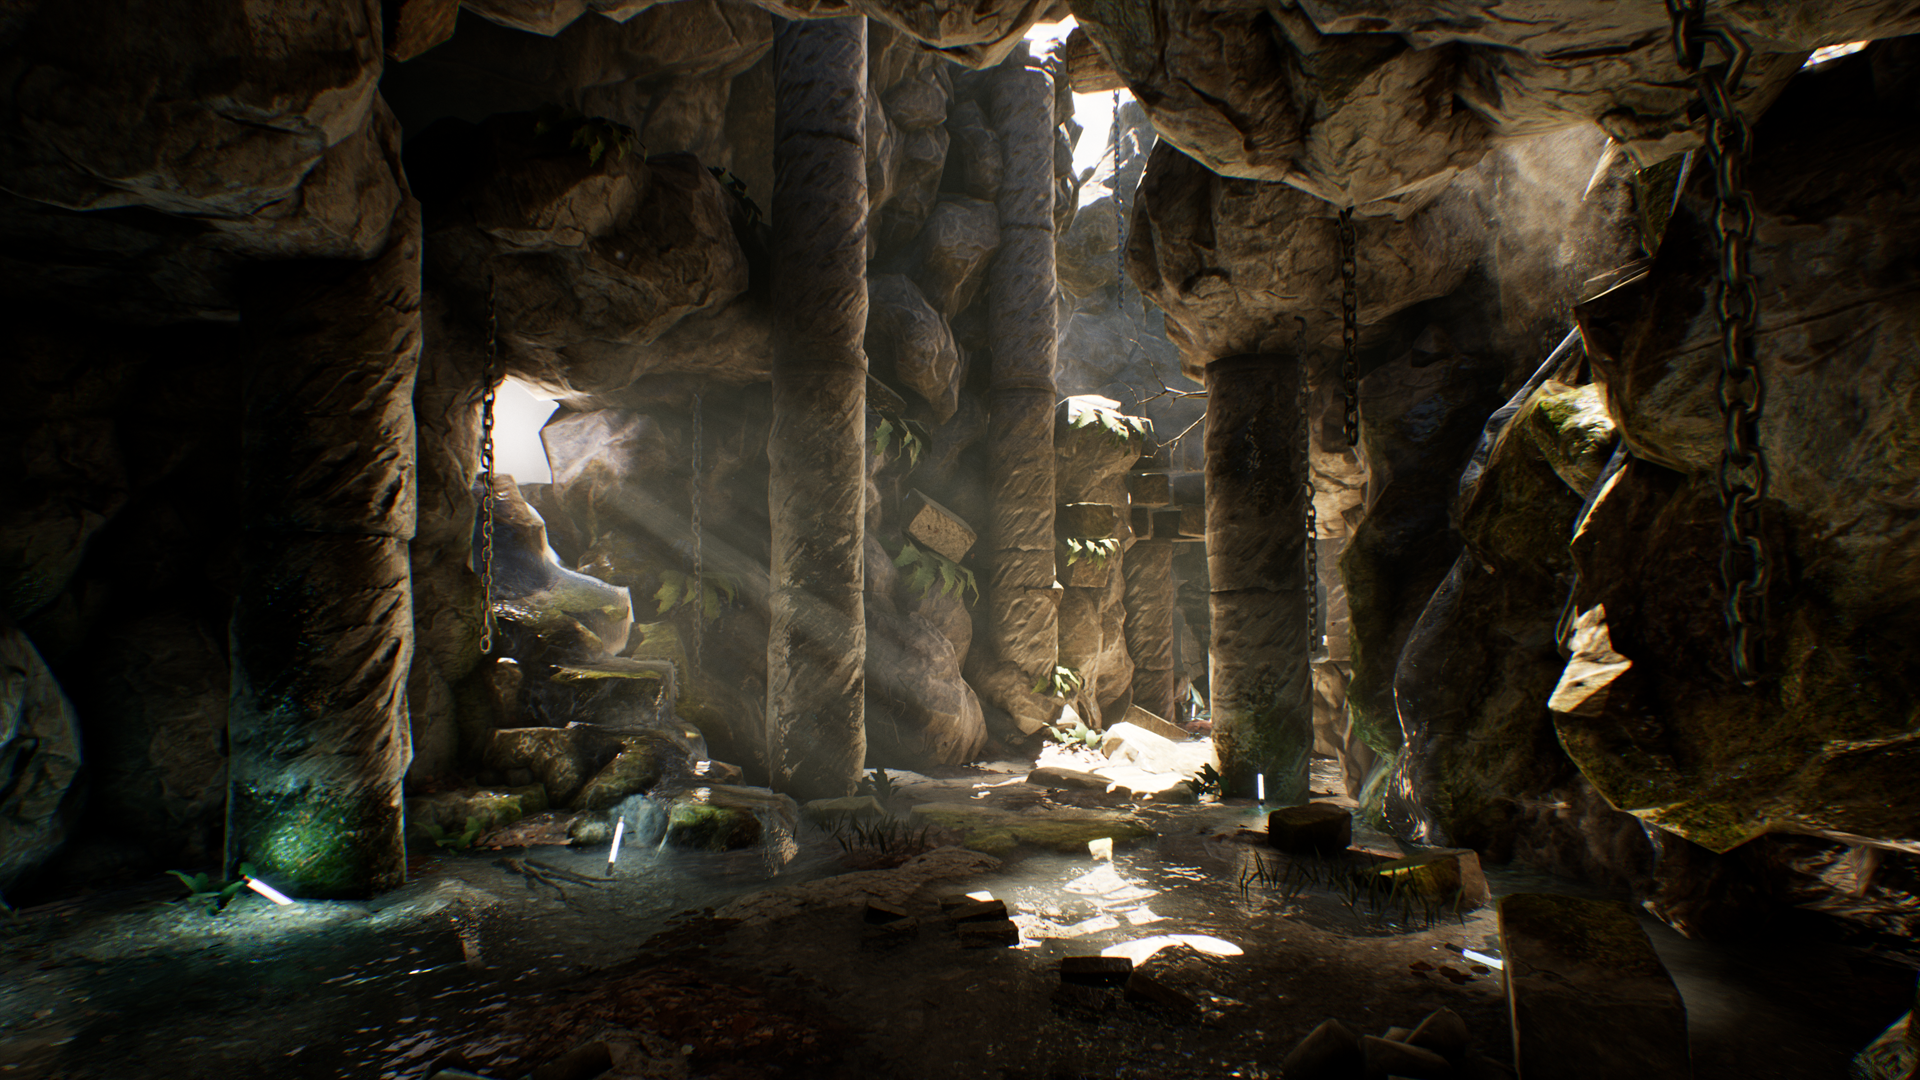
\includegraphics[scale=0.1]{environments/cave.png}

The following environments are only available in Windows
(therefore no significant experiments were done, but usage is possible).

\begin{enumerate}
    \item City.
    \item Africa.
    \item Jing-Zha.
    \item Neighborhood.
\end{enumerate}

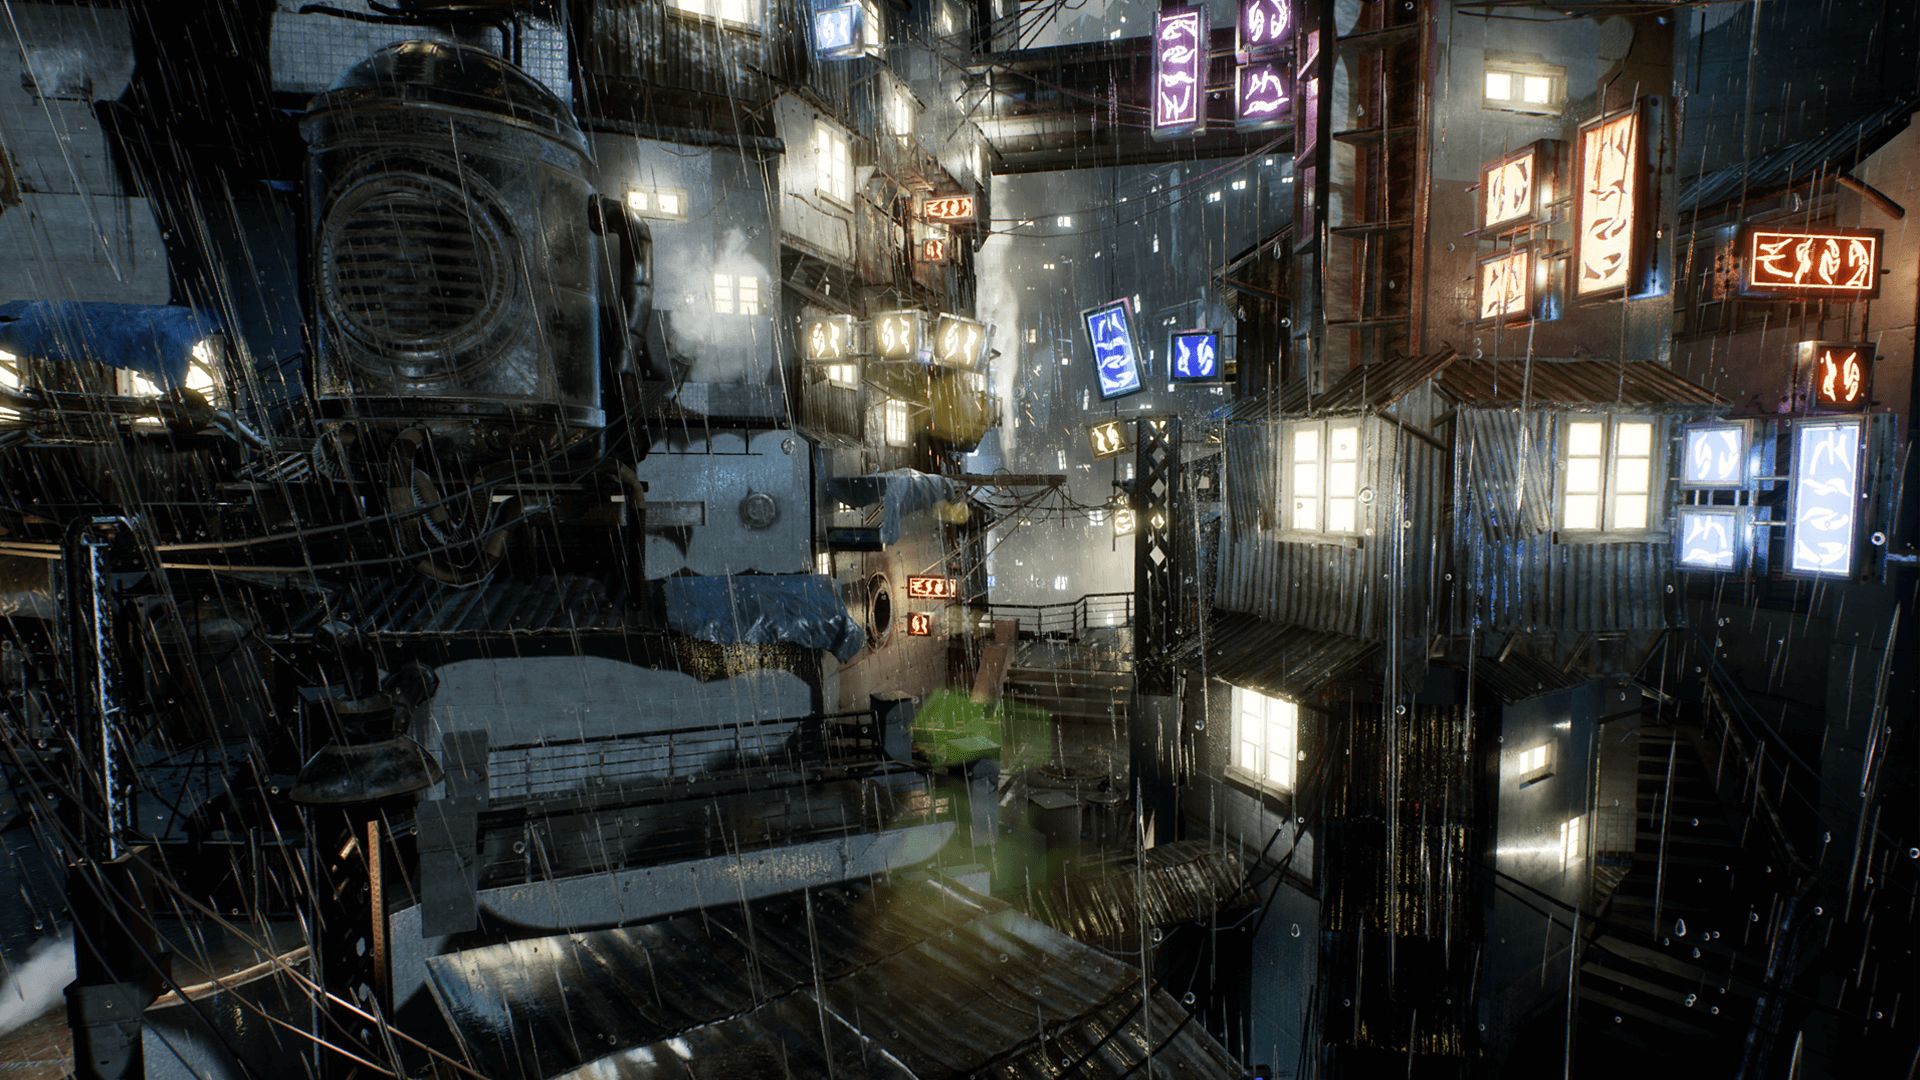
\includegraphics[scale=0.1]{environments/city.png}
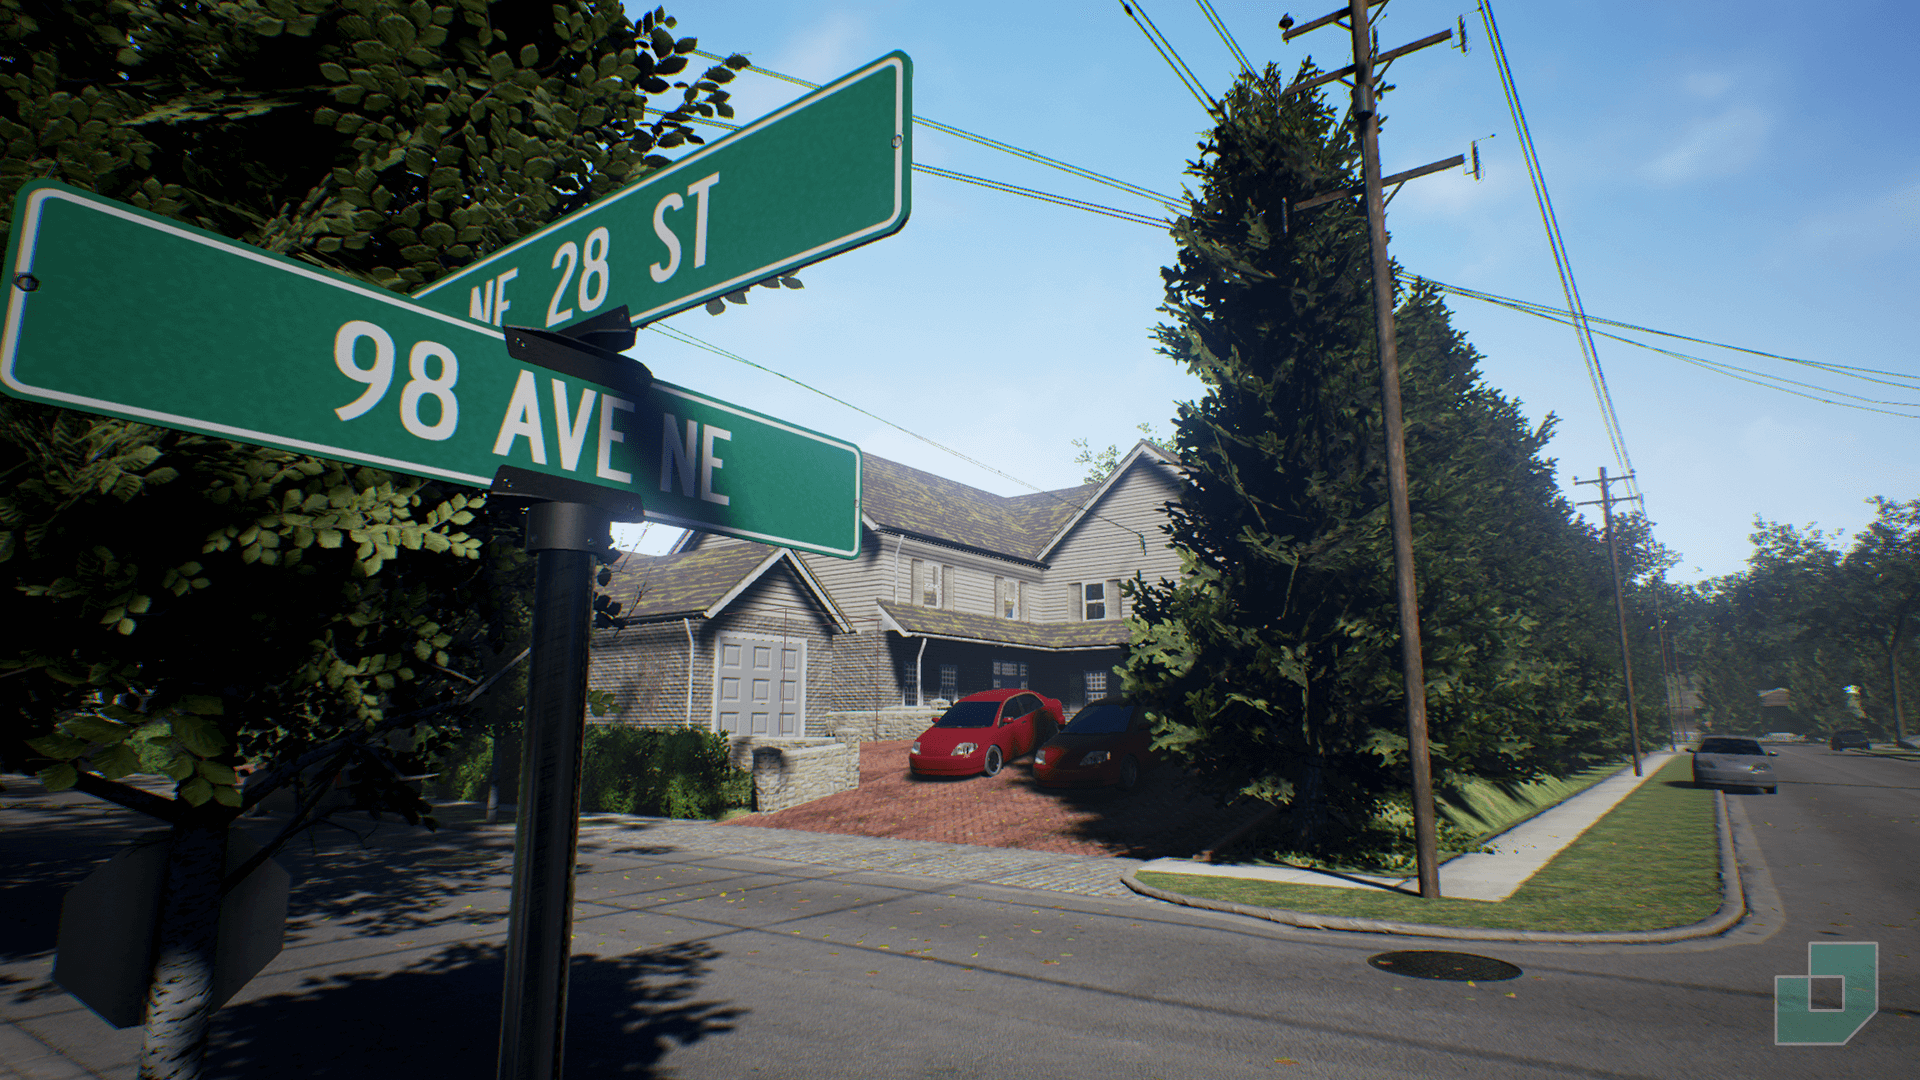
\includegraphics[scale=0.1]{environments/neighborhood.png}


\section{Agent: Deep Q-learning}

\subsection{General description}

We are based on the deep reinforcement
Q-learning, which was first described in \cite{mnih2013playing}.
After a while, more sophisticated version was published in
\cite{mnih2015humanlevel}.

 To use reinforcement learning successfully in situations
approaching real-world complexity, however, agents are confronted
with a difficult task: they must derive efficient representations of the
environment from high-dimensional sensory inputs, and use these
to generalize past experience to new situations. Remarkably, humans
and other animals seem to solve this problem through a harmonious
combination of reinforcement learning and hierarchical sensory pro-
cessing systems, the former evidenced by a wealth of neural data
revealing notable parallels between the phasic signals emitted by
dopaminergic neurons and temporal difference reinforcement learning
algorithms. Recent advances in training deep neural networks allow to
develop an artificial agent, termed a deep Q-network, that can
learn successful policies directly from high-dimensional sensory inputs
using end-to-end reinforcement learning.

To train the network, standard Q-learning update is converted into the
following loss:

$$L(\theta_i) = \mathbb{E}_{s,a,r,s'} \left[ \left(r + \gamma \max_{a'}Q(s', a'; \theta^{-}) - Q(s, a; \theta_i) \right)^2 \right] $$

\subsection{Network architecture}

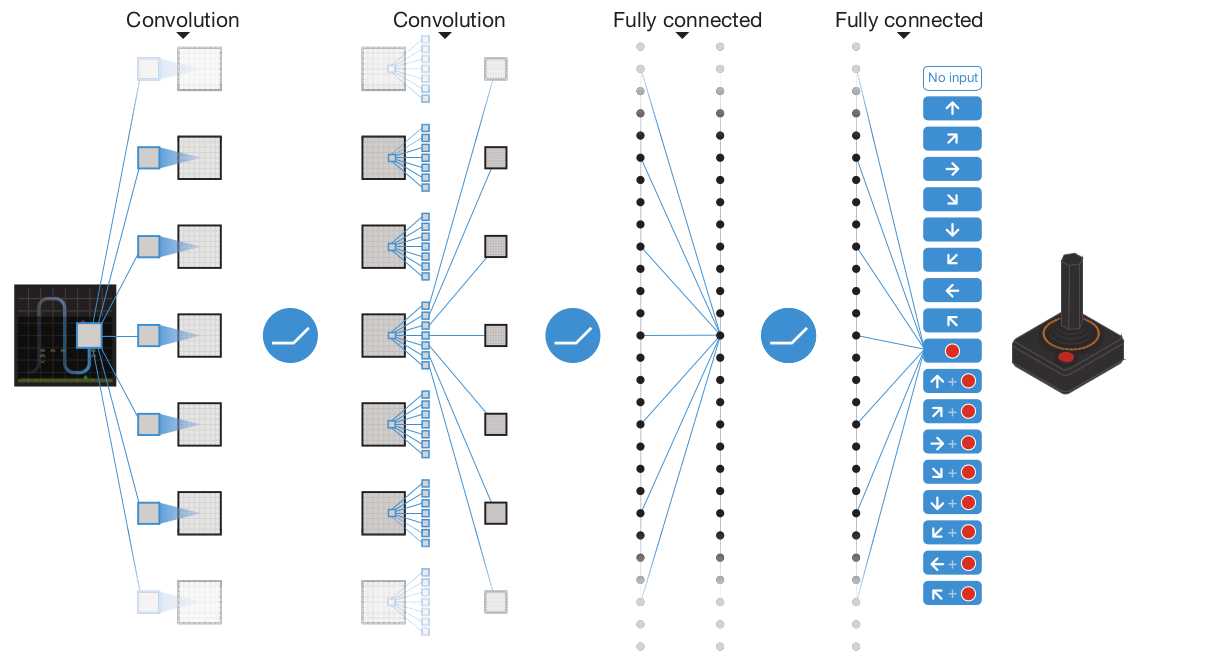
\includegraphics[scale=0.3]{dqn_crop.png}

\subsection{Applied tweaks}

\begin{itemize}
    \item {\bf Experience Replay.} History was collected, and experience was randomly sampled. That helped to reduce correlation in learning.
    \item {\bf Freezed network to reduce correlation.} When computing updates, freezed version was used for estimation. This helps
        to reduce bang of weights.
    \item {\bf Huber Loss.} Huber loss is more robust
        to outliars than MSE.
    \item {\bf 4-frame delayed learning.}
        Taking into account several frames helps network to understand
        distance, velocity and acceleration better.
\end{itemize}

\section{Implemented Rewards}

\begin{itemize}
    \item {\bf Exploration Reward.} Reward is described as $\frac{d - r}{\tau - r}$, where $d$ is distance, $r$ is radius, $\tau$ is constant.
        Also we penalize going too high.
    \item {\bf Path Reward.} We force collision avoidance to fixed lines, and penalize going far wary from them.
    \item {\bf Landscape Reward.} The aim is to reach the goal point in the environment. Therefore the reward is the difference $\text{dist}_{\text{prev}} - \text{dist}$ where $\text{dist}_{\text{prev}}$ is the distance to the goal in the previous state and $\text{dist}$ is distance to the goal in the current state. 
    \item {\bf Corridor Reward.}
\end{itemize}

\section{Implemented Action Spaces}

\begin{itemize}
    \item {\bf Grid Action Space.} Frontal camera image is separated into $M^2$ parts, which correspond to moving actions. Moving forward is
        mandatory.
    \item {\bf Canonical (Default) Action Space.} Forward, Backward, Up, Down, Left, Right, Stay.
    \item {\bf Flat Action Space.} No up or down, rotations introduced.
    \item {\bf Corridor Action Space.}
\end{itemize}

\section{Exploration}

\begin{itemize}
    \item {\bf Constant $\varepsilon$-greedy.} Exploration is constant over time, or disabled (for evaluation).
    \item {\bf Simulated annealing $\varepsilon$-greedy.} Exploration is scheduled by simulated annealing, and essentially decreases with time.
        Schedule is exponential.
\end{itemize}

\section{Results}

\section{Team Contribution}

The following parts were introduced:

\begin{enumerate}
    \item {\bf Project Proposal:} Aliaksandr Nekrashevich
    \item {\bf Architecture:} Aliaksandr Nekrashevich, Aibek Alanov
    \item {\bf Deep Agent Reproduction:} Aliaksandr Nekrashevich, Aibek Alanov, Dmitriy Salnikov
    \item {\bf AirSim tweaks:} Aliaksandr Nekrashevich, Dmitriy Salnikov
    \item {\bf Unreal Engine:} Dmitriy Salnikov, Aibek Alanov
    \item {\bf Windows Environment Adaptation:} Dmitriy Salnikov, Aibek Alanov
    \item {\bf Team Management:} Aliaksandr Nekrashevich
    \item {\bf Rewards:} Aliaksandr Nekrashevich, Aibek Alanov, Dmitriy Salnikov
    \item {\bf Action Spaces:} Aibek Alanov, Dmitriy Salnikov, Aliaksandr Nekrashevich
    \item {\bf Exploration Strategies:} Aibek Alanov, Dmitriy Salnikov
    \item {\bf Report:} Aliaksandr Nekrashevich, Aibek Alanov
    \item {\bf Presentation:} Aibek Alanov, Dmitriy Salnikov
\end{enumerate}

This is per-person separation:

\begin{itemize}
    \item {\bf Aibek Alanov.} Architecture of the framework, Deep Agent reproduction,
        Adopting Unreal Engine to Linux, Landscape Mountains environemt,
        Landscape Reward, Flat Action Space, Constant and Annealing exploration,
        Report, Presentation.

    \item {\bf Aliaksandr Nekrashevich.} Project proposal, Achitecture of
        the framework, Deep Agent reproduction, Blocks Environment,
        Corridor Environment, Exploration and Path Rewards,
        Grid and Default Action Spaces, Report, Team Management.

    \item {\bf Dmitriy Salnikov.} Deep Agent reproduction, AirSim Tweaks,
        Unreal Engine on Windows, Environment convertation to Linux,
        Environment hand-crafting, Corridor Reward, Cave and Corridor
        Environments, Windows Environments, Exploration Strategies,
        Presentation.
\end{itemize}

Team emphasises opinion of {\bf equal contribution} to this project from
each member.

\bibliographystyle{unsrt}
\bibliography{reference}

\end{document}
